% =============================================================================================
\chapter{Solution déployée}\label{chap:solution}

La solution est une application web Streamlit, déployée sur Streamlit Community Cloud à partir du dépôt GitHub, aux
couleurs de l'École Centrale Casablanca. Elle ne se limite pas à présenter nos 40 projets : n'importe quel jeu de
projets peut y être importé et évalué avec ses propres critères, poids, filtres et budget.

% ---------------------------------------------------------------------------------------------
\section{Fonctionnement}

L'application ne fait qu'\emph{afficher} des résultats et déclencher des calculs déterministes. Les résultats du
pipeline (projets, modèle entraîné, métriques, figures, paramètres) sont calculés à l'avance et versionnés dans le
dépôt, ce qui permet de démarrer sans base de données ni données brutes. Au premier passage, l'application évalue la
démonstration (environ 4 secondes, robustesse comprise) et met le résultat en cache. L'analyse active vit dans la
mémoire de session de chaque visiteur : si un utilisateur importe son propre jeu, les autres continuent de voir la
démonstration. La clé du modèle de langage est stockée dans les secrets de la plateforme et n'apparaît jamais dans le
code ni dans les messages.

\begin{figure}[htbp]
\centering
\begin{tikzpicture}[font=\small,
  box/.style={draw=eccgris,rounded corners=3pt,align=center,minimum height=0.95cm,fill=white},
  arr/.style={-{Stealth[length=2mm]},eccgris,thick}]
  \node[box,text width=4.2cm] (user) at (0,0) {\textbf{Utilisateur}\\ navigateur web};
  \node[box,text width=4.2cm] (gh) at (8,0) {\textbf{Dépôt GitHub}\\ code et résultats};
  \node[box,text width=9.2cm] (app) at (2.5,-1.9) {\textbf{app.py et pages} : affichage, 8 pages, barre latérale};
  \node[box,text width=9.2cm,draw=eccvert,line width=1pt,fill=eccclair] (state) at (2.5,-3.3)
       {\textbf{Analyse active} : jeu de projets, configuration, résultats (session et cache)};
  \node[box,text width=4.4cm] (eng) at (0.1,-4.9) {\textbf{Moteur}\\ filtre, MCDA, arbitrage};
  \node[box,text width=4.4cm] (ia) at (4.9,-4.9) {\textbf{IA}\\ agent rédacteur, conseiller};
  \node[box,text width=9.2cm] (files) at (2.5,-6.4) {\textbf{Fichiers du pipeline} : projets, modèle, métriques, figures};
  \node[box,text width=2.6cm] (gem) at (9.0,-4.9) {\textbf{Gemini}\\ API, clé secrète};
  \begin{scope}[on background layer]
    \node[draw=eccgris,dashed,rounded corners=5pt,fit=(app)(state)(eng)(ia)(files),inner sep=8pt,
          label={[text=eccgris,font=\scriptsize]north east:Streamlit Community Cloud}] {};
  \end{scope}
  \draw[arr,{Stealth[length=2mm]}-{Stealth[length=2mm]}] (user) -- (user|-app.north);
  \draw[arr] (gh) -- node[right,font=\scriptsize,text=eccgris]{à chaque mise à jour} (gh|-app.north);
  \draw[arr] (app) -- (state);
  \draw[arr] (state.south-|eng.north) -- (eng);
  \draw[arr] (state.south-|ia.north) -- (ia);
  \draw[arr] (files.north-|eng.south) -- (eng);
  \draw[arr] (ia) -- (gem);
\end{tikzpicture}
\caption{Architecture de l'application : les pages affichent, le moteur calcule, le modèle de langage ne fait que
rédiger.}
\label{fig:archi-app}
\end{figure}

% ---------------------------------------------------------------------------------------------
\section{Les pages de l'application}

\paragraph{Tableau de bord.} Six cartes de chiffres clés, une carte des projets selon deux critères au choix avec les
seuils du filtre, le classement ELECTRE III et un tableau filtrable et téléchargeable de tous les projets, avec leurs
critères, leurs rangs et les indicateurs de fragilité (figure~\ref{fig:app-dashboard}).

\begin{figure}[htbp]
  \centering
  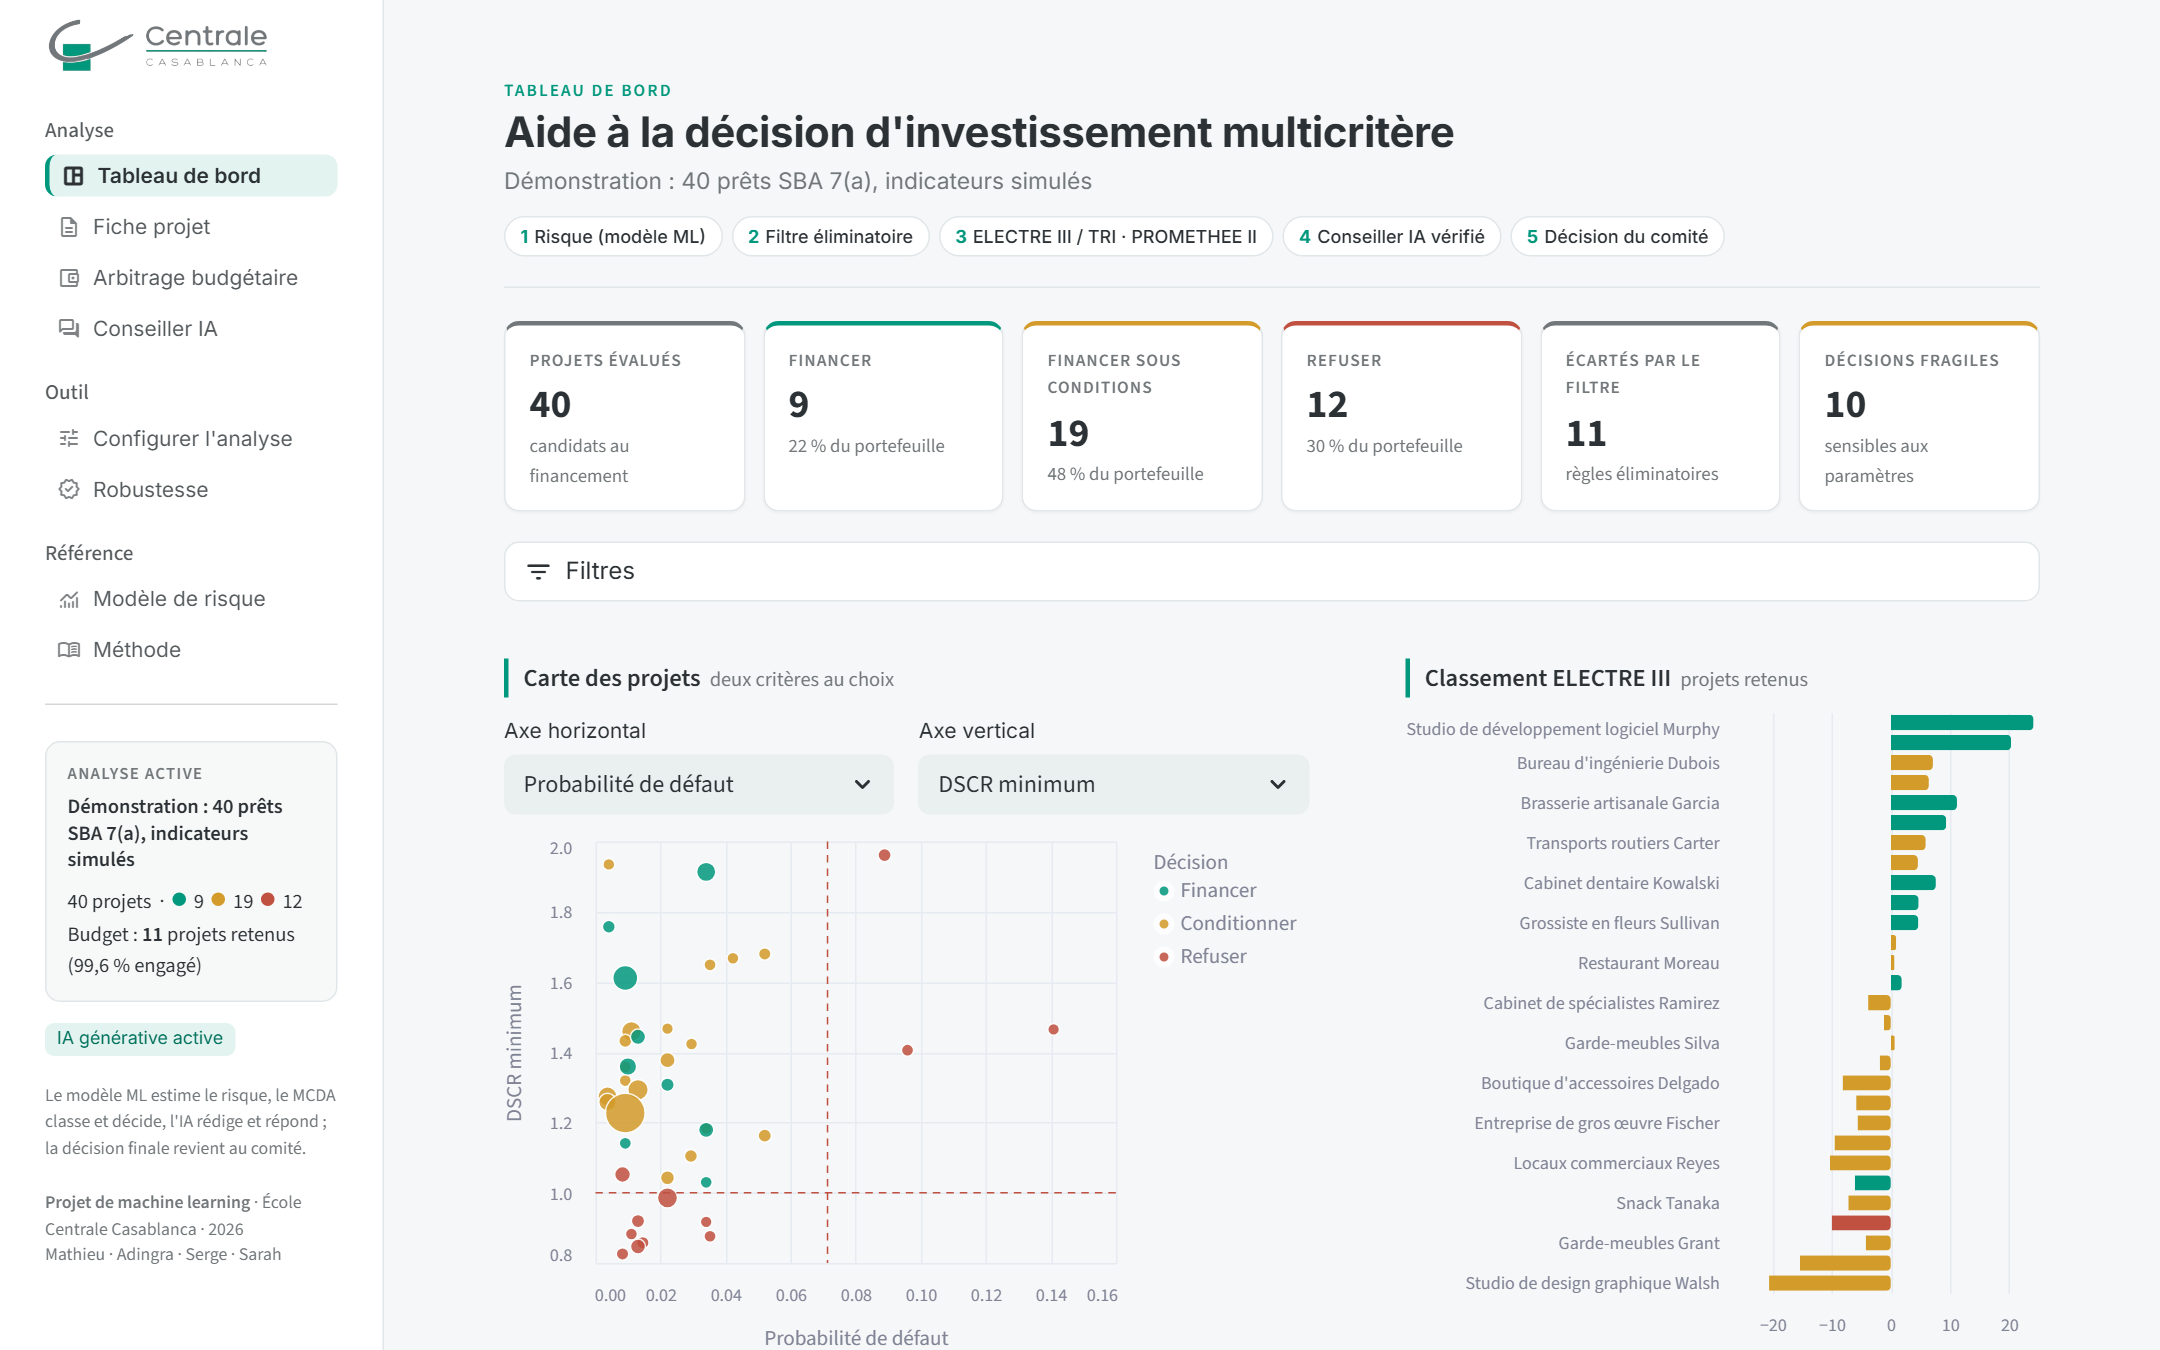
\includegraphics[width=\textwidth]{app_tableau_de_bord.png}
  \caption{Tableau de bord de l'application.}
  \label{fig:app-dashboard}
\end{figure}

\paragraph{Fiche projet.} Pour un projet choisi : sa catégorie, ses rangs, son statut budgétaire, puis un graphique
qui situe chaque critère par rapport aux profils d'ELECTRE TRI (zones Refuser, Conditionner, Financer), les facteurs
de risque issus de l'EBM, la fragilité et la note de l'agent rédacteur (figure~\ref{fig:app-fiche}). On y voit d'un
coup d'œil pourquoi le Cabinet dentaire Baker n'est que \og sous conditions \fg{} : risque, ESG et levier dans la zone
verte, VAN, délai et emplois dans la zone rouge.

\begin{figure}[htbp]
  \centering
  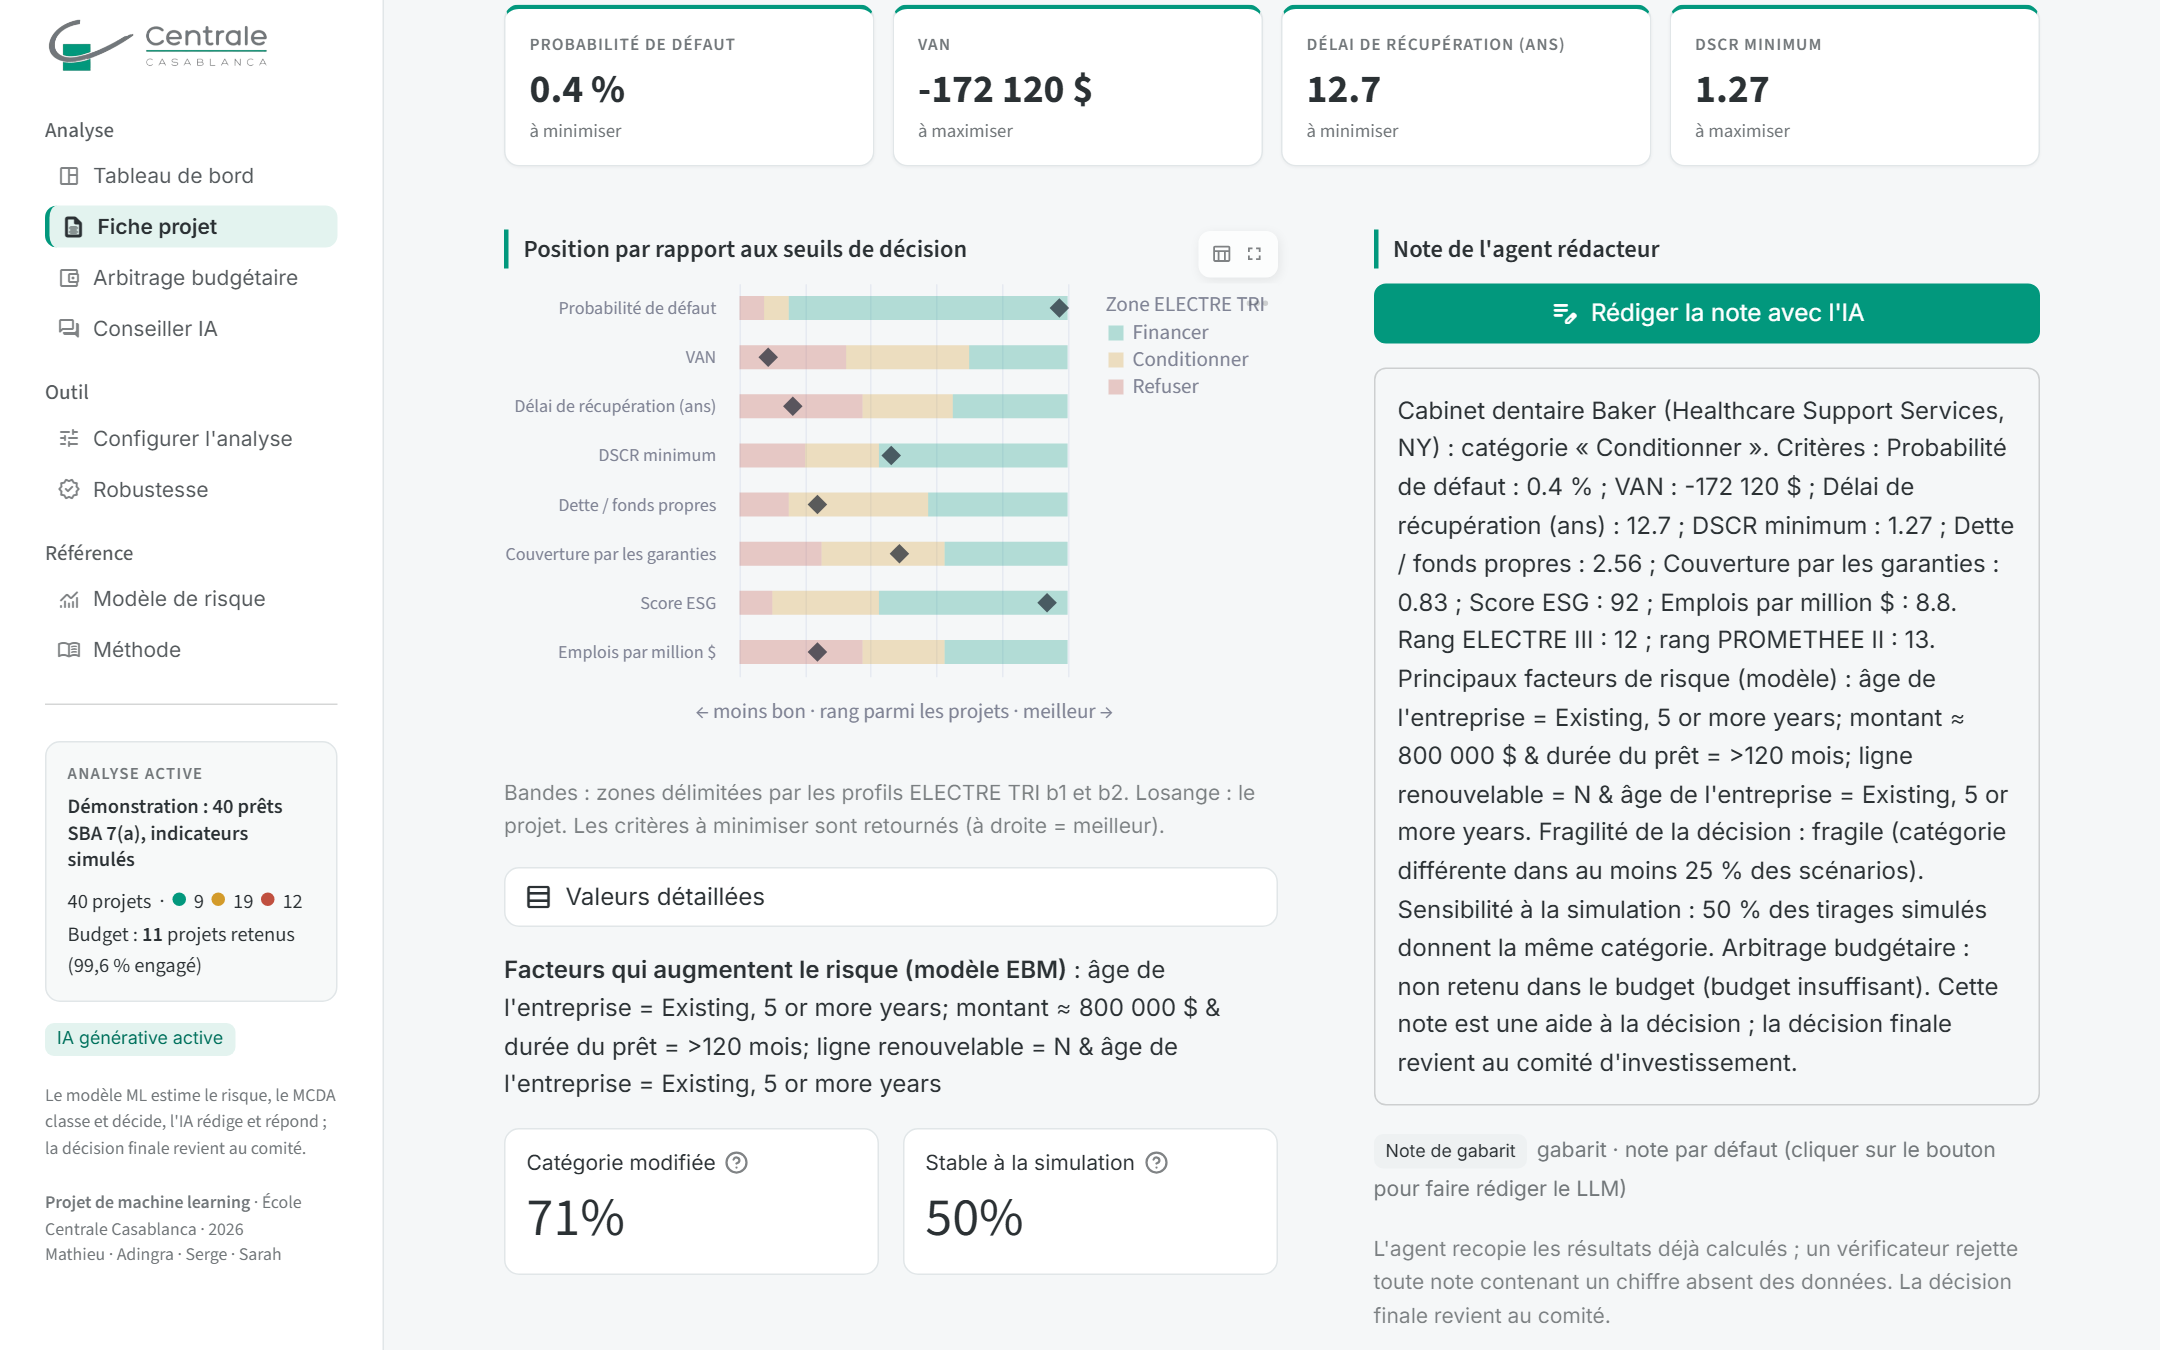
\includegraphics[width=\textwidth]{app_fiche_projet.png}
  \caption{Fiche projet du Cabinet dentaire Baker : position par rapport aux seuils et note de l'agent.}
  \label{fig:app-fiche}
\end{figure}

\paragraph{Arbitrage budgétaire.} Les paramètres du comité (budget, bornes, plafond sectoriel, inclusion des projets
sous conditions, règle de sélection) se règlent en direct ; la page montre le montant engagé, les secteurs financés,
les motifs de non-sélection et la décision projet par projet (figure~\ref{fig:app-arbitrage}).

\begin{figure}[htbp]
  \centering
  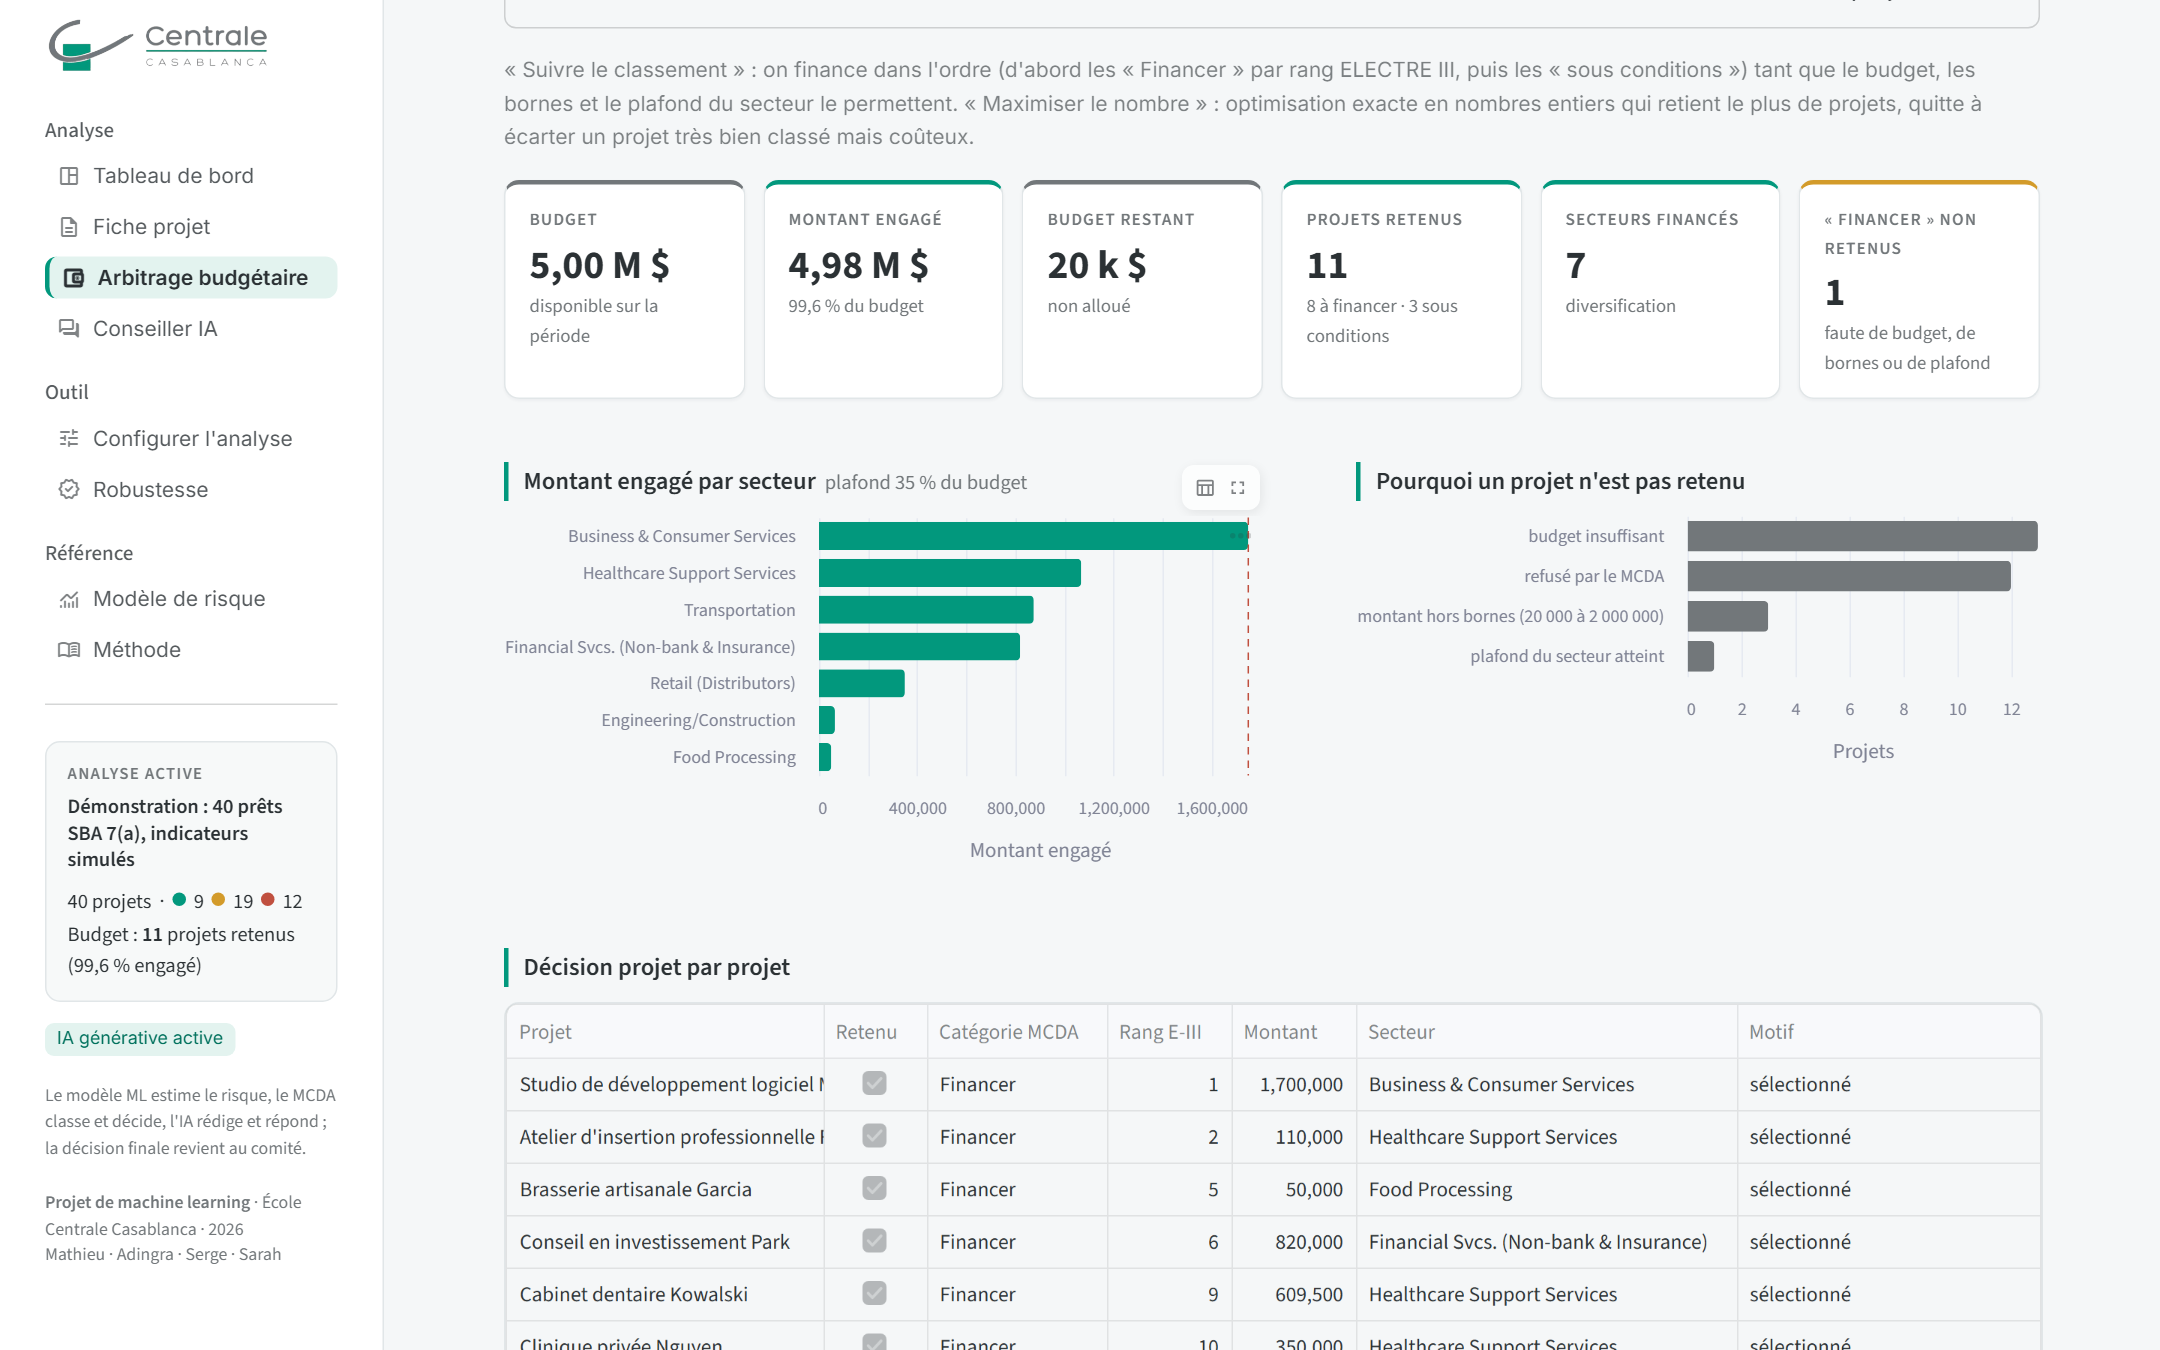
\includegraphics[width=\textwidth]{app_arbitrage.png}
  \caption{Arbitrage budgétaire : chiffres clés, montant par secteur et motifs de non-sélection.}
  \label{fig:app-arbitrage}
\end{figure}

\paragraph{Conseiller IA.} On pose une question en français ; le conseiller appelle ses outils et rédige une réponse
dont les nombres sont vérifiés. La figure~\ref{fig:app-conseiller} montre la réponse à la question \og Donne-moi les
détails du projet Garde-meubles Silva si l'ESG pèse 20\,\% et la VAN 30\,\% \fg{} : le conseiller a relancé le MCDA
avec ces poids, constaté que le projet passe de \og sous conditions \fg{} à \og Financer \fg{} (rang 17 à 15), et
signale que tous ses chiffres viennent des données consultées.

\begin{figure}[htbp]
  \centering
  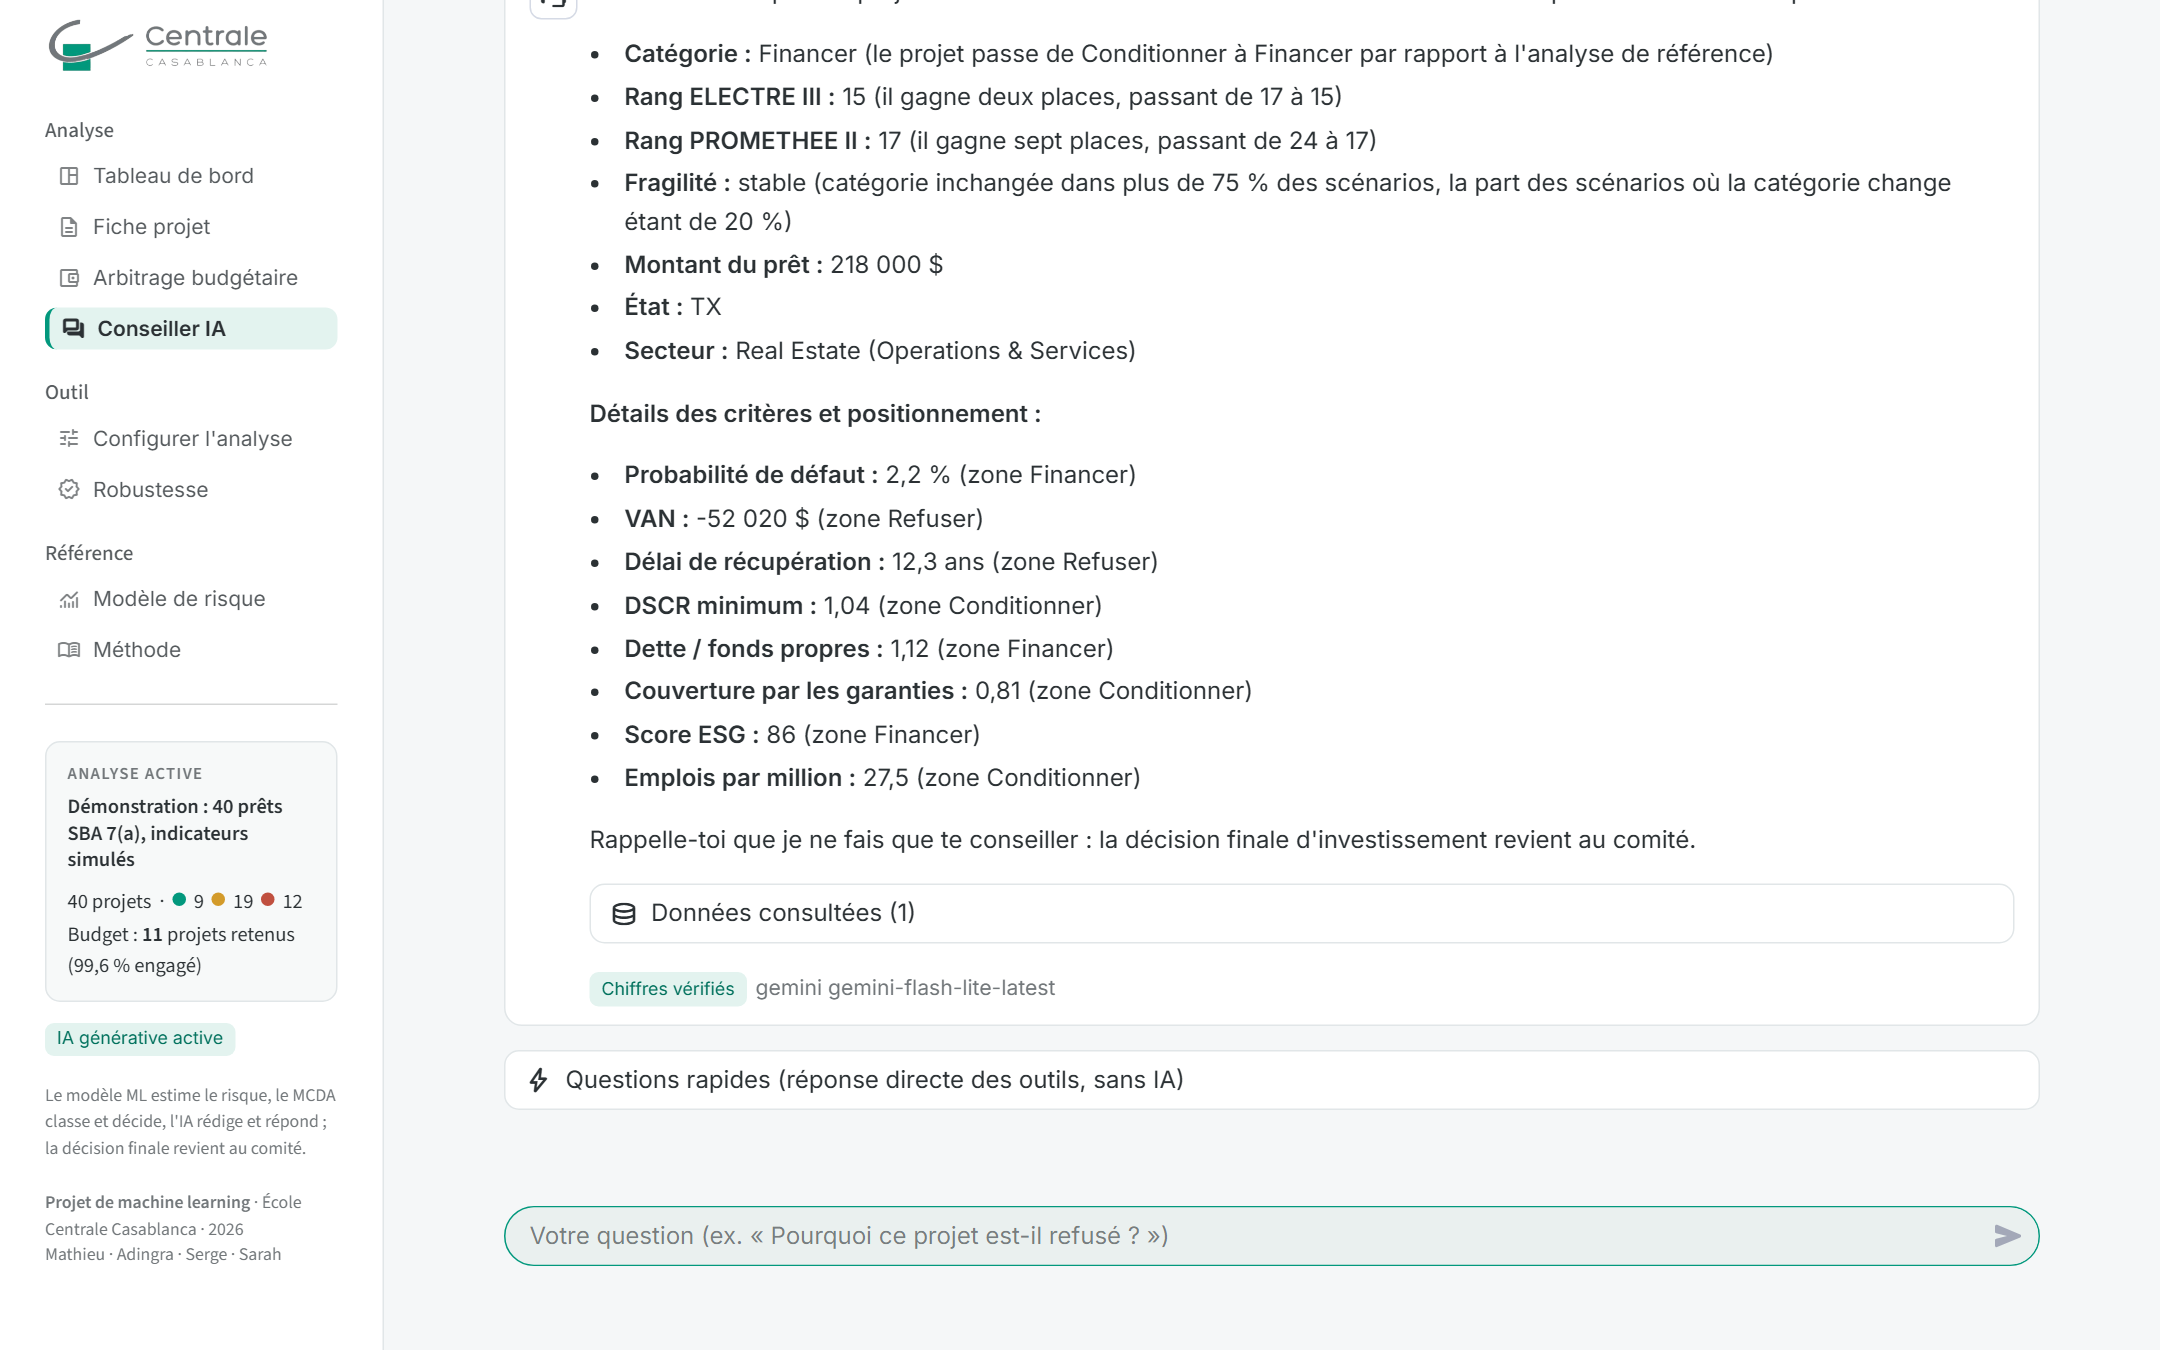
\includegraphics[width=\textwidth]{app_conseiller.png}
  \caption{Réponse du conseiller IA à une question de scénario, avec l'étiquette \og Chiffres vérifiés \fg{}.}
  \label{fig:app-conseiller}
\end{figure}

\paragraph{Configurer l'analyse, Robustesse, Modèle de risque, Méthode.} Les quatre autres pages permettent de
configurer une nouvelle analyse (section suivante), d'examiner la sensibilité des décisions, de consulter les
performances et les explications du modèle de risque, et de lire la méthode avec ses paramètres actifs et ses limites.

% ---------------------------------------------------------------------------------------------
\section{Un outil réutilisable}

La page \og Configurer l'analyse \fg{} transforme la démonstration en outil (figure~\ref{fig:app-config}) :

\begin{enumerate}
  \item \textbf{données} : import d'un fichier CSV ou Excel, une ligne par projet ; les nombres écrits à la française
        sont reconnus ; si le fichier décrit des prêts au format SBA sans probabilité de défaut, le modèle de risque la
        calcule ;
  \item \textbf{critères} : choix des colonnes, du libellé, du sens (deviné d'après le nom : un coût, un risque ou un
        délai est à minimiser), du poids et des profils $b_1$ et $b_2$ ;
  \item \textbf{pondération} : poids saisis ou AHP, avec la matrice des comparaisons et le ratio de cohérence
        affiché en direct ;
  \item \textbf{filtre} : autant de règles \og colonne, opérateur, seuil \fg{} que voulu ;
  \item \textbf{ELECTRE} : seuils $q$, $p$, $v$ et coupure $\lambda$.
\end{enumerate}
Tant qu'une erreur subsiste (valeur manquante, poids nuls, AHP incohérent), un message l'explique et le calcul est
bloqué. La configuration s'enregistre et se recharge en JSON, et la même évaluation est disponible en ligne de
commande. Quatre jeux de test fictifs accompagnent l'outil : 15 PME du Grand Casablanca en dirhams avec une
configuration AHP, 10 prêts au format SBA, 8 projets d'énergie avec des critères entièrement différents (taux de
rendement interne, coût par mégawatt, CO$_2$ évité, risque pays) et un fichier volontairement erroné.

\begin{figure}[htbp]
  \centering
  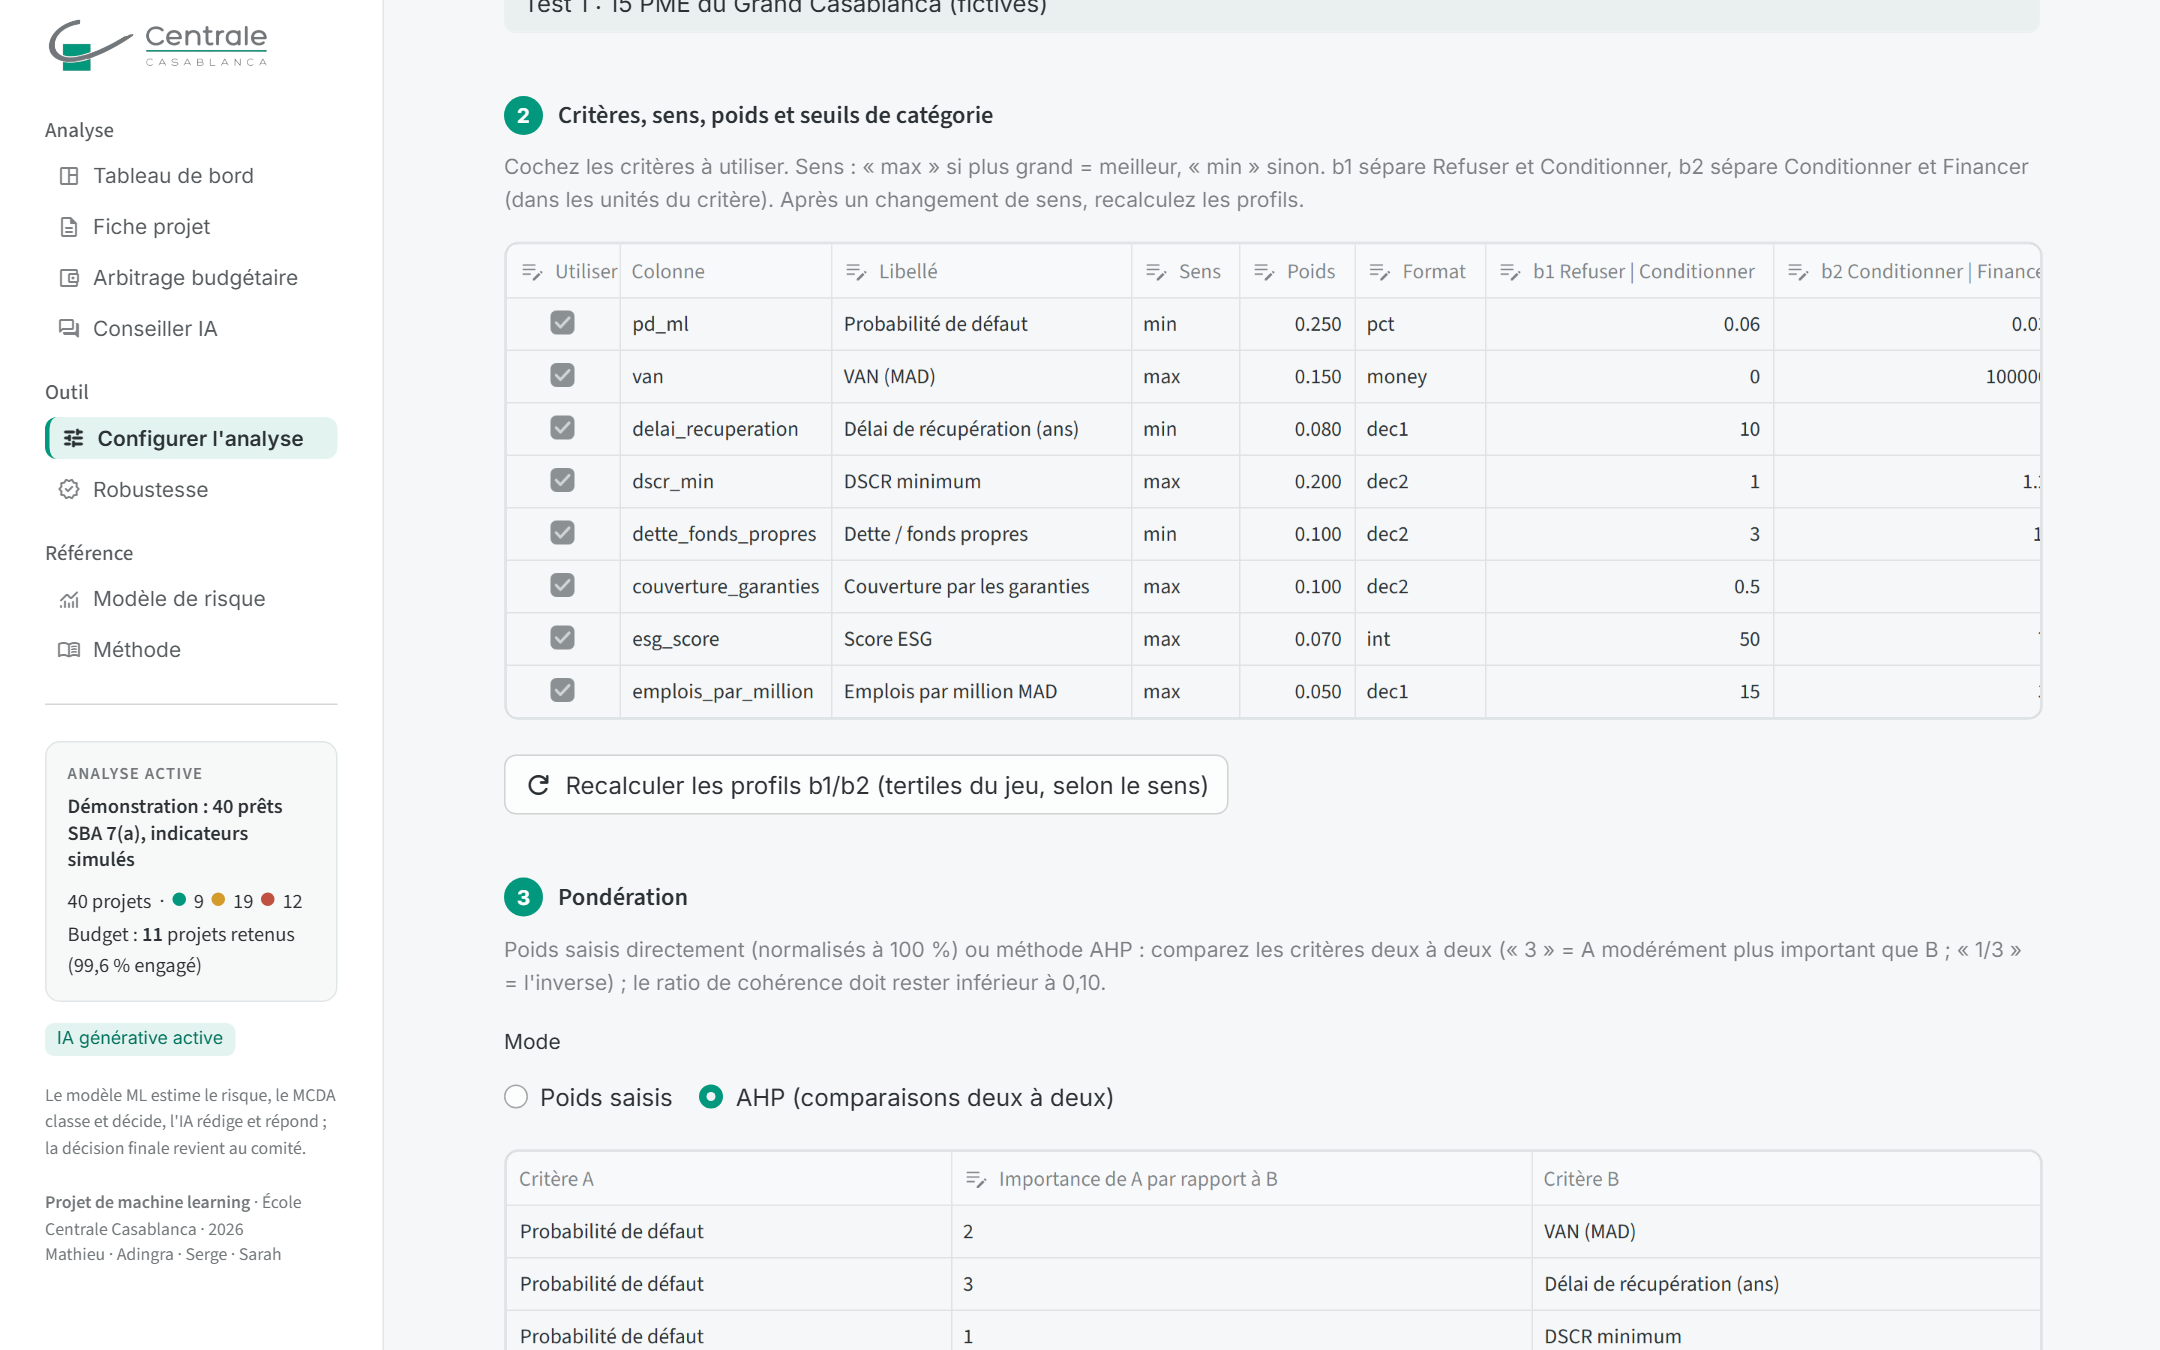
\includegraphics[width=\textwidth]{app_configurer.png}
  \caption{Page de configuration après import d'un jeu de 15 PME : tableau des critères, sens, poids et profils.}
  \label{fig:app-config}
\end{figure}

% ---------------------------------------------------------------------------------------------
\section{Reproductibilité et qualité}

Le dépôt GitHub contient le code source (\code{src/}), l'application (\code{app/}), les notebooks d'exploration et
de modélisation, les petits fichiers de résultats et un README qui décrit l'installation, l'ordre d'exécution, le
journal des données (source, taille, date) et chaque choix. Les données brutes, trop volumineuses, n'y sont pas : un
script vérifie leur présence et indique leurs adresses de téléchargement. Tous les tirages aléatoires ont une graine
fixe : deux exécutions donnent les mêmes chiffres. Trente tests automatiques vérifient notamment :

\begin{itemize}
  \item un exemple ELECTRE à trois projets calculé à la main (concordance, veto, classement) ;
  \item l'absence de variables qui fuient ou font double compte, et l'indépendance de la simulation vis-à-vis de
        l'issue réelle ;
  \item que le moteur générique reproduit exactement les résultats du pipeline sur la démonstration ;
  \item que l'arbitrage respecte toujours le budget, les bornes et le plafond sectoriel, pour les deux règles ;
  \item les outils du conseiller et la détection des chiffres et des méthodes inventés.
\end{itemize}
